\documentclass{beamer}
\usetheme{Madrid}
\usepackage[utf8]{inputenc}
\usepackage{amsmath, amssymb}
\usepackage{graphicx}

\title{Poiseuille Flow: Analytical and Numerical Study}
\author{Masud}
\date{\today}

\begin{document}

% Title
\begin{frame}
\titlepage
\end{frame}

% Outline
\begin{frame}{Outline}
\tableofcontents
\end{frame}

% Introduction
\section{Introduction}
\begin{frame}{Flow Configuration}
Poiseuille flow describes laminar flow of a viscous fluid driven by a pressure gradient in a confined geometry.

\begin{itemize}
    \item Steady, incompressible, and fully developed
    \item Common geometries:
    \begin{itemize}
        \item Flow between two parallel plates
        \item Flow inside a circular pipe
    \end{itemize}
\end{itemize}

Governing equations (steady-state, incompressible):
\[
\begin{aligned}
\rho (\mathbf{u} \cdot \nabla)\mathbf{u} &= -\nabla p + \mu \nabla^2 \mathbf{u}, \\
\nabla \cdot \mathbf{u} &= 0
\end{aligned}
\]
\end{frame}

% Analytical Solution
\section{Analytical Solution}
\begin{frame}{Analytical Solution}
For 2D plane Poiseuille flow between two plates $y = 0$ and $y = H$:

\[
\frac{d^2 u}{dy^2} = \frac{1}{\mu} \frac{dp}{dx}, \qquad u(0) = u(H) = 0
\]

Integrating twice:
\[
u(y) = \frac{1}{2\mu} \frac{dp}{dx} \, (y^2 - Hy)
\]

\begin{itemize}
    \item Parabolic velocity profile
    \item Maximum velocity at mid-plane: \( u_{max} = -\frac{H^2}{8\mu} \frac{dp}{dx} \)
\end{itemize}
\end{frame}

% Numerical Method
\section{Numerical Method}
\begin{frame}{Discretization}
\begin{itemize}
    \item Discretize in $y$ using second-order central differences
    \item Solve linear system:
    \[
    -u_{j-1} + 2u_j - u_{j+1} = \frac{(\Delta y)^2}{\mu} \frac{dp}{dx}
    \]
    \item Apply boundary conditions: \( u_0 = u_N = 0 \)
    \item Solve using matrix inversion or iterative methods (Jacobi, Gauss-Seidel)
\end{itemize}
\end{frame}

% Example
\section{Example}
\begin{frame}{Comparison of Results}
\begin{figure}[h]
\centering
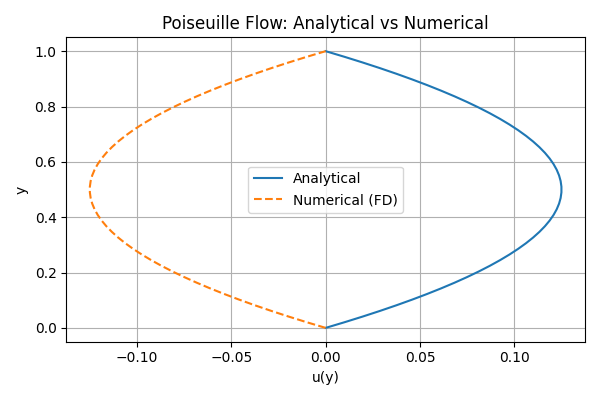
\includegraphics[width=0.8\linewidth]{poiseuille_plot.png} % replace with your figure
\caption{Velocity profile for plane Poiseuille flow: analytical vs. numerical}
\end{figure}
\end{frame}

% Discussion
\section{Discussion}
\begin{frame}{Observations}
\begin{itemize}
    \item Numerical solution matches analytical parabolic profile
    \item Higher grid resolution improves accuracy
    \item Benchmark case for testing viscous solvers and discretization accuracy
\end{itemize}
\end{frame}

% Conclusion
\section{Conclusion}
\begin{frame}{Conclusion}
\begin{itemize}
    \item Poiseuille flow demonstrates viscous, laminar motion under pressure gradient
    \item Analytical solution serves as a validation test for CFD solvers
    \item Numerical methods capture the parabolic velocity distribution efficiently
\end{itemize}
\end{frame}

\end{document}